\documentclass{article}

%%%%%%%%%%%%%%%%%%%%%%%%%%%%%%
%% 1. Document Class Setup
%%%%%%%%%%%%%%%%%%%%%%%%%%%%%%
% Before accepting by the NeurIPS conference, select one of the options below.
% 1. "main" option is used for the Main Track
% \usepackage[main]{neurips_2026}
% \usepackage[main, final]{neurips_2026}
% "preprint" option is used for arXiv or other preprint submissions
 % \usepackage[preprint]{neurips_2026}
% to avoid loading the natbib package, add option nonatbib:
%    \usepackage[nonatbib]{neurips_2026}
\usepackage[main, final]{neurips_2026}



%%%%%%%%%%%%%%%%%%%%%%%%%%%%%%
%% 2. Import Settings & Packages
%%%%%%%%%%%%%%%%%%%%%%%%%%%%%%
\input{math_commands.tex}

%%%%%%%%%%%%%%%%%%%%%%%%%%%%%%
%% 1. Graphics and Color Handling
%%%%%%%%%%%%%%%%%%%%%%%%%%%%%%
% Support for including graphics (images, plots)
\usepackage{graphicx} 

% Support for color management (text color, background color)
\usepackage{xcolor}

% Advanced color management for tables (row/column shading)
\usepackage{colortbl}

% Create colored and framed text boxes (fancy boxes for highlights)
\usepackage[most]{tcolorbox}

%%%%%%%%%%%%%%%%%%%%%%%%%%%%%%
%% 2. Tables and Figures
%%%%%%%%%%%%%%%%%%%%%%%%%%%%%%
% Professional quality tables (improves spacing and rules)
\usepackage{booktabs}

% Support for multi-row cells in tables
\usepackage{multirow}

% Adjust content size (scale, rotate, clip boxes)
\usepackage{adjustbox}

% Advanced cell formatting (line breaks within cells)
\usepackage{makecell}

% Auto-width tables (columns that fill available width)
\usepackage{tabularx}

% Tables that span multiple pages
\usepackage{longtable}

% Extended array and tabular environments
\usepackage{array}

% Support for subfigures (figures within figures)
\usepackage{subcaption}

% Wrap text around figures and tables
\usepackage{wrapfig} 

%%%%%%%%%%%%%%%%%%%%%%%%%%%%%%
%% 3. Typography and Formatting
%%%%%%%%%%%%%%%%%%%%%%%%%%%%%%
% Input encoding support (UTF-8)
\usepackage[utf8]{inputenc} 

% Micro-typographic extensions (improves spacing and kerning)
\usepackage[patch=none]{microtype}

% Customizing captions in floating environments
% Note: Commented out because subcaption already handles caption customization.
% \usepackage{caption}

% Allow double-column floats at the bottom of pages
\usepackage{stfloats}

% Line numbering (useful for review process)
\usepackage{lineno}

% Additional symbols (text symbols like copyright, registered trademark)
\usepackage{textcomp}

% Font encoding (OT1 for compatibility)
\usepackage[OT1]{fontenc} 

% Balance columns on the last page of two-column documents
\usepackage{balance}

% Customizing lists (enumerate, itemize)
\usepackage{enumitem} 

% Nice fractions (e.g., 1/2 instead of 1 over 2)
\usepackage{nicefrac}       

%%%%%%%%%%%%%%%%%%%%%%%%%%%%%%
%% 4. Math and Logic
%%%%%%%%%%%%%%%%%%%%%%%%%%%%%%
% AMS math packages (essential for advanced math typesetting)
\usepackage{amsmath}
\usepackage{amsfonts}
\usepackage{amssymb}
\usepackage{bm}       % Bold math symbols

% Theorem environments (theorems, lemmas, proofs)
\usepackage{amsthm}

% Dingbat symbols (checkmarks, crosses, etc.)
\usepackage{pifont}

%%%%%%%%%%%%%%%%%%%%%%%%%%%%%%
%% 5. Algorithms and Code
%%%%%%%%%%%%%%%%%%%%%%%%%%%%%%
% NOTE: 'algorithm2e' is commented out because 'icml2026.sty' already loads 'algorithm' and 'algorithmic'.
% Enabling it here causes a "Command \algorithm already defined" error.
% \usepackage[ruled,linesnumbered]{algorithm2e}

% NOTE: 'algpseudocode' is also incompatible with the default 'algorithmic' package loaded by 'icml2026.sty'.
% \usepackage{algpseudocode}

% Source code listing (syntax highlighting)
\usepackage{listings}

% Verbatim environment (for raw text output)
\usepackage{verbatim}

%%%%%%%%%%%%%%%%%%%%%%%%%%%%%%
%% 6. Navigation and Hyperlinks
%%%%%%%%%%%%%%%%%%%%%%%%%%%%%%
% Support for hyperlinks (citations, URLs, cross-references)
% Note: Usually loaded last to avoid conflicts.
\usepackage{hyperref}

% Attempt to make hyperref and algorithmic work together better:
\newcommand{\theHalgorithm}{\arabic{algorithm}}

%%%%%%%%%%%%%%%%%%%%%%%%%%%%%%
%% 7. Development and Review
%%%%%%%%%%%%%%%%%%%%%%%%%%%%%%
% Insert 'to-do' items and comments in the document (useful for drafts)
% Option 'textsize=tiny' makes the note text small.
% You can add 'disable' to the options to hide all notes (e.g., [disable,textsize=tiny])
\usepackage[textsize=tiny]{todonotes}

%%%%%%%%%%%%%%%%%%%%%%%%%%%%%%
%% Reference
%%%%%%%%%%%%%%%%%%%%%%%%%%%%%%
% cleveref must be set after the hyperref
\usepackage[capitalize,noabbrev]{cleveref}




%%%%%%%%%%%%%%%%%%%%%%%%%%%%%%
%% 1. Table and Figure Settings
%%%%%%%%%%%%%%%%%%%%%%%%%%%%%%
% Format subfigure captions.
% Result: Separates label and caption with a space; sets 1pt vertical skip.
% Note: If "Unused \captionsetup[subfigure]" warning occurs, subcaption package might be missing or conflicting. Keep commented if unused.
%\captionsetup[subfigure]{labelsep=space, skip=1pt}

%%%%%%%%%%%%%%%%%%%%%%%%%%%%%%
%% 2. Algorithm Customizations
%%%%%%%%%%%%%%%%%%%%%%%%%%%%%%
% Note: The following settings rely on 'algorithm2e'.
% Since 'icml2026.sty' loads conflicting packages by default, we have commented out algorithm2e in packages.tex.
% Therefore, these settings must also be commented out to avoid errors.

% Define 'Input' keyword
% Result: Displays "Input: " in algorithms.
% \SetKwInput{KwInput}{Input}

% Define 'Output' keyword
% Result: Displays "Output: " in algorithms.
% \SetKwInput{KwOutput}{Output}

% Define 'Block' comment style
% Result: Uses '⊳' symbol for inline comments.
% \SetKwComment{Block}{$\triangleright$\ }{}

% Attempt to fix compatibility between hyperref and algorithmic
% \newcommand{\theHalgorithm}{\arabic{algorithm}}

% Define standard comment style
% Result: Uses '//' for comments.
% \SetKwComment{Comment}{//  }{}

% Prevent automatic semicolon printing
% Result: No semicolons automatically added at line ends.
% \DontPrintSemicolon

% Customize 'if-else' structure
% Result: Sets display keywords for If, ElseIf, Else.
% \SetKwIF{If}{ElseIf}{Else}{if}{}{else if}{else}{end if}%

%%%%%%%%%%%%%%%%%%%%%%%%%%%%%%
%% 3. Highlighting and Colors
%%%%%%%%%%%%%%%%%%%%%%%%%%%%%%
% Define line highlighting command \HiLi
% Result: Creates a light gray background for the current line (useful for emphasizing table rows).
\def\HiLi{\leavevmode\rlap{\hbox to \hsize{\color{gray!20}\leaders\hrule height .8\baselineskip depth .5ex\hfill}}}

% Define dark blue color
\definecolor{darkblue}{rgb}{0, 0, 0.5}

% Configure hyperlink colors
% Result: Citations, internal links, and URLs appear in dark blue and are clickable in PDF.
\hypersetup{
  colorlinks=true,   % Enable colored links
  citecolor=darkblue, % Color for citations (e.g., [1])
  linkcolor=darkblue, % Color for internal links (e.g., Figure 1)
  urlcolor=darkblue   % Color for external URLs
}

%%%%%%%%%%%%%%%%%%%%%%%%%%%%%%
%% 4. Code Listings Configuration
%%%%%%%%%%%%%%%%%%%%%%%%%%%%%%
% Configure 'listings' package display
\lstset{
  basicstyle=\ttfamily\footnotesize,       % Font: Monospaced, footnote size
  breaklines=true,                         % Line breaking: Auto-wrap long lines
  breakatwhitespace=false,                 % Break at: Allow breaks at any character, not just spaces
  showstringspaces=false,                  % String spaces: Do not show visible markers for spaces in strings
  columns=flexible,                        % Alignment: Flexible character width to avoid awkward spacing
  frame=single,                            % Frame: Add a single-line frame around code blocks
  backgroundcolor=\color{lightgray!20}     % Background: Light gray background for code blocks
}

%%%%%%%%%%%%%%%%%%%%%%%%%%%%%%
%% 5. Theorem and Proof Environments
%%%%%%%%%%%%%%%%%%%%%%%%%%%%%%
% Set theorem style to 'plain'
% Result: Bold title, italic body (for core statements like Theorems, Lemmas)
\theoremstyle{plain}

% Define 'theorem' environment
% Result: Numbered by section (e.g., Theorem 1.1)
\newtheorem{theorem}{Theorem}[section]

% Define 'proposition' environment
% Result: Shares numbering with Theorem (e.g., Proposition 1.2)
\newtheorem{proposition}[theorem]{Proposition}

% Define 'lemma' environment
% Result: Shares numbering with Theorem (e.g., Lemma 1.3)
\newtheorem{lemma}[theorem]{Lemma}

% Define 'corollary' environment
% Result: Shares numbering with Theorem (e.g., Corollary 1.4)
\newtheorem{corollary}[theorem]{Corollary}

% Set theorem style to 'definition'
% Result: Bold title, upright body (for Definitions, Assumptions)
\theoremstyle{definition}

% Define 'definition' environment
% Result: Shares numbering with Theorem
\newtheorem{definition}[theorem]{Definition}

% Define 'assumption' environment
% Result: Shares numbering with Theorem
\newtheorem{assumption}[theorem]{Assumption}

% Set theorem style to 'remark'
% Result: Italic title, upright body (for Remarks)
\theoremstyle{remark}

% Define 'remark' environment
% Result: Shares numbering with Theorem
\newtheorem{remark}[theorem]{Remark}





%%%%%%%%%%%%%%%%%%%%%%%%%%%%%%
%% 3. Title
%%%%%%%%%%%%%%%%%%%%%%%%%%%%%%
\title{Interpretable Financial Market Simulation with Large Model-Based Multi-Agent Systems }


%%%%%%%%%%%%%%%%%%%%%%%%%%%%%%
%% 4. Authors
%%%%%%%%%%%%%%%%%%%%%%%%%%%%%%
%%%%%%%%%%%%%%%%%%%%%%%%%%%%%%
%% Authors Configuration
%%%%%%%%%%%%%%%%%%%%%%%%%%%%%%
% The \author macro works with any number of authors. There are two commands
% used to separate the names and addresses of multiple authors: \And and \AND.
%
% Using \And between authors leaves it to LaTeX to determine where to break the
% lines. Using \AND forces a line break at that point. So, if LaTeX puts 3 of 4
% authors names on the first line, and the last on the second line, try using
% \AND instead of \And before the third author name.

\author{%
  Mingxian Ke \\
  ID: 50033277\\
  The Hong Kong University of Science and Technology (Guangzhou)\\
  \texttt{mke517@connect.hkust-gz.edu.cn} \\
  % examples of more authors
  % \And
  % Coauthor \\
  % Affiliation \\
  % Address \\
  % \texttt{email} \\
}



\begin{document}


\maketitle


\begin{abstract}
This study aims to systematically analyze the functional architecture of multi-agent financial market simulation codebases. By leveraging sample cases from the examples directory, we seek to understand the simulation workflows and underlying mechanisms of different agent architectures. Building upon this foundation, we select a specific scenario for empirical analysis to better identify the strengths and limitations of Large Language Models (LLMs) in financial simulations. Ultimately, this research provides methodological guidance and empirical support for constructing an interpretable, interactive financial sandbox model oriented toward decision-makers.
\end{abstract}

%%%%%%%%%%%%%%%%%%%%%%%%%%%%%%
%% Section 1: Introduction
%%%%%%%%%%%%%%%%%%%%%%%%%%%%%%
\section{Research Background and Problem Statement}
\label{sec:intro}

Traditional financial models exhibit significant limitations. These models rely on mathematical formulas and simplified frameworks for decision-making, possessing limited information processing capabilities. Consequently, they fail to address complex real-world financial scenarios, adapt to evolving market structures, or accommodate unexpected events. Moreover, traditional financial models tend to be highly stylized and idealized, thereby overlooking individual heterogeneity and cognitive biases.

Traditional financial market simulation models suffer from fundamental deficiencies in interpretability. Although capable of generating plausible trading sequences or price trajectories, researchers remain unable to ascertain why agents make specific decisions at particular moments. This absence of transparency leads to two critical consequences: (i) inability to perform causal attribution—when abnormal fluctuations occur in simulations, researchers cannot trace the underlying causes; and (ii) constrained model diagnosis and iteration—when simulation performance is suboptimal, researchers can only adjust parameters or network structures blindly without direct access to agents' reasoning chains.


%%%%%%%%%%%%%%%%%%%%%%%%%%%%%%
%% Section 2: Research Objectives
%%%%%%%%%%%%%%%%%%%%%%%%%%%%%%
\section{Research Objectives}
\label{sec:objectives}

This study aims to systematically analyze the functional architecture of multi-agent financial market simulation codebases. By leveraging sample cases from the examples directory, we seek to understand the simulation workflows and underlying mechanisms of different agent architectures. Building upon this foundation, we select a specific scenario for empirical analysis to better identify the strengths and limitations of Large Language Models (LLMs) \cite{qwen2.5-analysis} in financial simulations. Ultimately, this research provides methodological guidance and empirical support for constructing an interpretable, interactive financial sandbox model oriented toward decision-makers.


%%%%%%%%%%%%%%%%%%%%%%%%%%%%%%
%% Section 3: LLM-Based Multi-Agent Systems
%%%%%%%%%%%%%%%%%%%%%%%%%%%%%%
\section{Composition and Execution Logic of LLM-Based Multi-Agent Systems}
\label{sec:system}

\subsection{Component Functions}
\label{subsec:components}

\subsubsection{Simulator}
\label{subsubsec:simulator}

The Simulator serves as the scheduling hub and state manager in the masim framework, responsible for driving temporal progression, environment state updates, and simulation parameter control in multi-agent systems.

\paragraph{Temporal Scheduling and Round Control.}
The Simulator drives the entire simulation process in discrete rounds, with each round representing a discrete time step. In each round, the Simulator sequentially triggers the following operations: loading current market data from the data source, broadcasting this data to all Players, awaiting decision results from each Player, aggregating action instructions, and updating the market environment. This mechanism ensures that all agents make decisions simultaneously based on identical external information, guaranteeing simulation reproducibility and comparability.

\paragraph{Environment State Management and Market Clearing.}
The Simulator assumes unified responsibility for maintaining the market environment. It manages global state variables in the simulation, such as current price and trading volume. After each Player returns trading instructions, the Simulator executes order matching and clearing logic: matching buy and sell orders, updating positions and cash balances, and adjusting market prices. This environment update process alters agents' perceptual inputs in the next round, forming a closed loop of ``perception-decision-action-feedback.''

\paragraph{Experimental Parameter Management and Logging.}
The Simulator provides centralized configuration interfaces for experimental parameters and logging functionality. Researchers configure simulation parameters---including agent quantity and types, initial market state, maximum simulation rounds, and transaction fees---through the Simulator's setup interface. During execution, the Simulator automatically records key events and state changes, including per-round market data snapshots, agent action records, order execution details, and final asset distributions. These log data support post-simulation metric calculation and visualized replay analysis.

\subsubsection{Persona}
\label{subsubsec:persona}

The Persona serves as the cognitive and decision-making core of agents in the masim framework, responsible for encapsulating agent identity characteristics, memory mechanisms, reasoning logic, and action generation.

\paragraph{Identity Characteristics and Initial State Configuration.}
The Persona defines an agent's role positioning and behavioral tendencies through a set of configurable identity attributes.

\subsubsection{Proxy}
\label{subsubsec:proxy}

\paragraph{Message Routing and Forwarding.}
The Proxy functions as the message bus between agents, responsible for receiving, parsing, and forwarding messages. All inter-agent communication must pass through the Proxy, which determines the destination of messages based on topology constraints and communication rules, ensuring information flows along predefined pathways.

\paragraph{Communication History Recording.}
The Proxy maintains a complete message history. All messages forwarded through the Proxy in each simulation round are recorded to structured storage, containing complete metadata including timestamps, senders, recipients, and message content. These historical records support post-simulation communication behavior analysis, such as information propagation path tracing, inference of opinion influence relationships among agents, and auditing of abnormal trading behaviors. Message history also provides external data sources for the Persona's memory module, enabling agents to review past communications for decision-making.

\paragraph{Message Format Specification and Filtering Mechanism.}
The Proxy handles message format specification and validity verification. All messages transmitted through the Proxy must conform to predefined message templates; the Proxy validates message format integrity before forwarding and rejects invalid or maliciously constructed messages. Furthermore, the Proxy supports configurable message filtering rules, enabling interception or flagging of specific messages based on sender identity, message type, or content keywords. This mechanism provides a controllable entry point for information intervention in simulation experiments.

\subsubsection{Topology}
\label{subsubsec:topology}

The Topology serves as the definer of communication relationships and information flow patterns among agents in the masim framework, responsible for constructing and maintaining structured connection relationships in the agent network.

\paragraph{Network Structure Definition and Connection Management.}
The Topology implements mathematical abstraction and instantiation management of agent communication networks. It defines directed or undirected connection relationships between agent nodes, supporting multiple classical network topology types. The Topology generates and initializes the connection matrix at simulation startup based on preset network parameters, and supports dynamic adjustment during execution. This structure defines the rule boundaries of ``who can send messages to whom'' among agents, serving as the core framework for simulating information propagation and social influence.

\paragraph{Information Propagation Path Control and Noise Injection.}
The Topology assumes control over message propagation paths in the agent network. When the Proxy performs message routing, the Topology provides current communication topology constraints: messages can only be transmitted along defined connection edges, with recipients limited to neighbor nodes with existing connections. The Topology also supports injecting propagation noise and attenuation mechanisms during message transmission, simulating information distortion and intensity decay in real-world social networks. This mechanism enables researchers to simulate diffusion patterns of information under heterogeneous network structures, such as rapid rumor propagation in tightly-knit communities and the formation of information silos.

\paragraph{Network Data Recording and Structural Property Computation.}
The Topology provides recording functionality for network operational data and real-time computation interfaces for structural metrics. It continuously records actual communication frequencies between agents, connection strength changes, and network dynamic evolution during simulation. Simultaneously, the Topology exposes computation methods for network structural metrics, including but not limited to: node degree distribution, average path length, clustering coefficient, modularity, and centrality indices. These metrics can be read by the Persona's perception module during simulation, enabling agents to be ``aware'' of their positional roles in the network and adjust their information processing strategies accordingly.

\subsubsection{Communication}
\label{subsubsec:communication}

The Communication is a core component in the multi-agent financial market simulation framework responsible for defining and constraining inter-agent information exchange behaviors, designed to accurately reproduce the structural characteristics of information asymmetry and information propagation in real financial markets.

\paragraph{Message Semantic Specification.}
To ensure information interoperability among heterogeneous agents driven by different underlying models, this module establishes standardized message payload structures. Each message contains message type, content body, confidence score, and timeliness marker. The module incorporates built-in format validation mechanisms; all messages with format anomalies or semantic mismatches are rejected from forwarding.

\paragraph{Communication Timing and Protocol Management.}
The module imposes strict temporal constraints on inter-agent information exchange. In terms of timing control, messages are restricted to exchange within designated communication rounds, with any form of communication prohibited during decision computation phases, thereby preventing agents from obtaining non-public information through instant Q\&A. Regarding interaction protocols, the module predefines multiple communication modes, including request-response, broadcast-subscription, and negotiation-consensus modes, with automatic management of complex multi-round dialogue state transitions. Furthermore, the module introduces a communication cost model, where each communication consumes a certain amount of ``communication budget,'' simulating the economic cost of information acquisition in real markets.

\paragraph{Identity Authentication and Access Control.}
The module maintains fine-grained send and receive permission lists: send permissions stipulate that agents of different roles may only send specific message types; receive permissions define the visibility scope of public and insider information. The communication module forms a clear division of labor with the network topology module: the topology module defines network structural constraints of ``who connects to whom,'' while the communication module defines content and role constraints of ``who can say what, who can hear what,'' with both collaborating to construct multi-layered information asymmetry environments.


\subsection{Execution Logic}
\label{subsec:execution}

The execution logic of the multi-agent system follows a structured phase-based pipeline. \Cref{tab:execution} summarizes the core operations, input sources, and output destinations for each component during execution.

\begin{table}[ht]
\centering
\caption{Execution logic of the multi-agent financial market simulation system.}
\label{tab:execution}
\resizebox{\textwidth}{!}{%
\begin{tabular}{@{}lllll@{}}
\toprule
\textbf{Component} & \textbf{Execution Phase} & \textbf{Core Operation} & \textbf{Input Source} & \textbf{Output Destination} \\
\midrule
Agent Module & Phase Execute & Receive info $\rightarrow$ reason $\rightarrow$ generate messages \& orders & Environment, Communication, Topology & Messages $\rightarrow$ Comm., Orders $\rightarrow$ Env. \\
Communication Module & Phase Dispatch & Validate $\rightarrow$ encode $\rightarrow$ route $\rightarrow$ deliver messages & Agent Module's output messages & Target agent's receive queue \\
Topology Module & Phase Dispatch & Determine message routing paths & Communication Module's encoded messages & Target node list \\
Environment Module & Init + Trade Exec. & Update market state, execute order matching & Agent Module's orders & Market data, portfolio updates \\
Logging Module & All phases & Record decisions, communications, trades, market state & All other components & Structured log data \\
Scheduler & All phases & Control round progression \& phase transitions & Time parameters & Execution signals to each component \\
\bottomrule
\end{tabular}%
}
\end{table}


%%%%%%%%%%%%%%%%%%%%%%%%%%%%%%
%% Section 4: Experiments
%%%%%%%%%%%%%%%%%%%%%%%%%%%%%%
\section{Analyzing Runtime Results of Different Models: A Case Study of Asset Bubbles}
\label{sec:experiments}

\subsection{RAG Model}
\label{subsec:rag}

% TODO: Add RAG model figure here
\begin{figure}[ht]
  \centering
  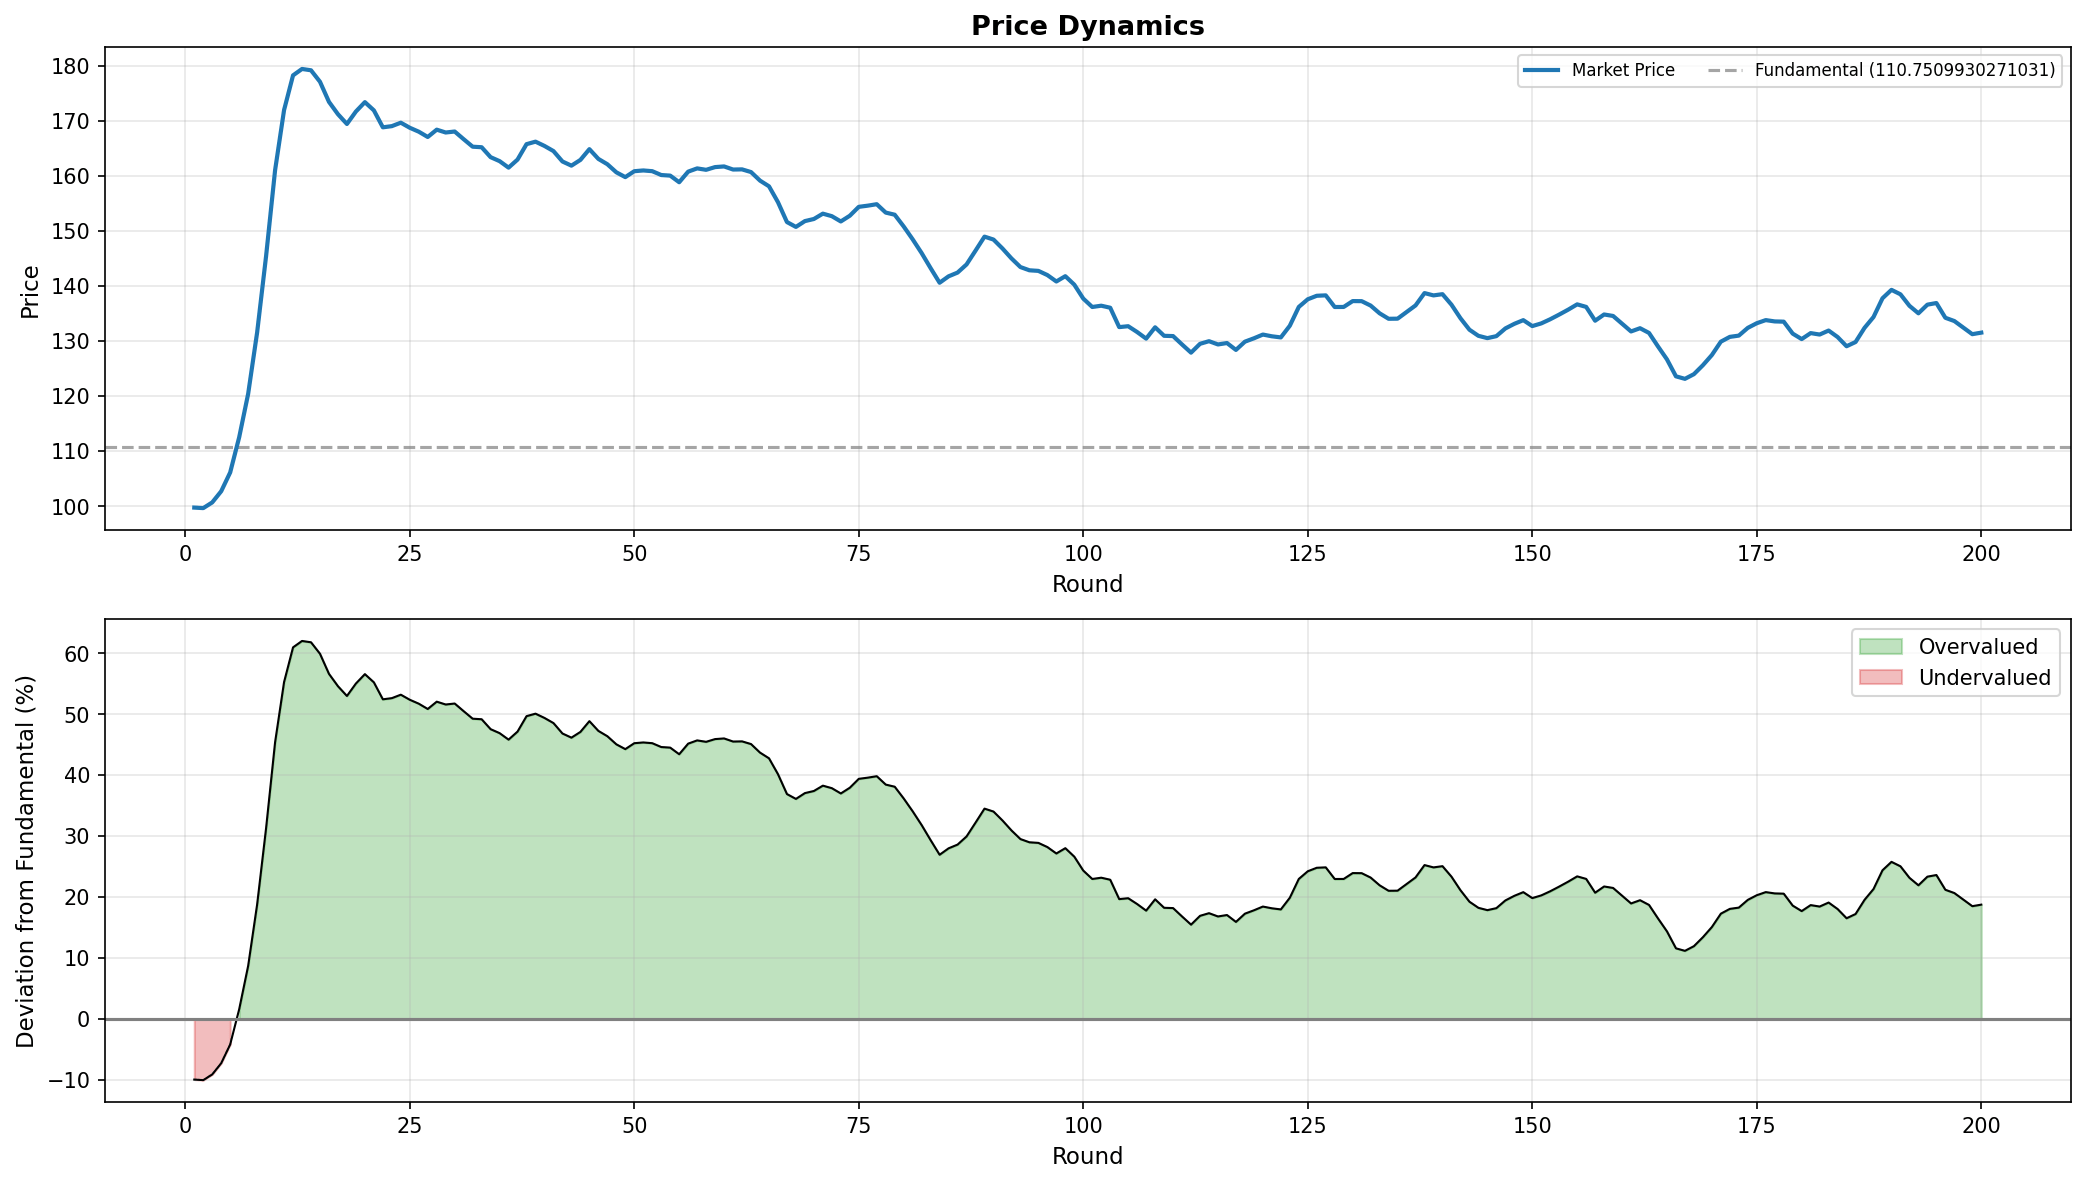
\includegraphics[width=\textwidth]{results/rag_results.jpg}
  \caption{Asset bubble simulation results using the RAG model.}
  \label{fig:rag}
\end{figure}

\paragraph{Results Analysis.}
The fundamental value is approximately 110. In the early market stage, the price hovers around 10\% below the fundamental value, followed by a pronounced acceleration in the initial phase. Within approximately the first 10 rounds, the price rapidly surges to near 180, forming significant price deviation. Compared to the fundamental value, the deviation magnitude expands rapidly during this stage, indicating strong non-fundamental-driven characteristics in the market---consistent with typical manifestations of asset bubble formation, namely ``price departing from fundamentals, deviation magnitude rising rapidly, and accompanied by short-term momentum enhancement.''

After reaching the peak, the price enters a phase of high-level oscillation and gradual decline. Although the price retreats from its peak, the decline is limited; the market does not exhibit ``rapid collapse'' or ``significant breach below fundamentals with sustained downward movement'' consistent with bubble bursting. From the deviation perspective, subsequent prices remain long-term in a range approximately 20\% above fundamentals, with the bubble state not fully subsiding.

Meanwhile, momentum and drawdown-related indicators in the model exhibit phase-dependent changes: upward price momentum strengthens during bubble formation, while in subsequent phases, although drawdowns and instability emerge, they fail to trigger sustained intense collapse processes. This result indicates that the market indeed undergoes critical stages of bubble establishment, but bubble bursting remains incomplete---manifested as slow decline in deviation levels and sluggish equilibrium reversion speed.

Overall, this simulation demonstrates that the market exhibits pronounced bubble characteristics in the initial phase, but fails to show rapid and thorough bubble liquidation in the later phase, ultimately forming a structure of ``long-term overvaluation with gradual reversion''---reflecting that bubble bursting conditions may be insufficiently triggered or that reversion mechanisms exhibit lag in this scenario. The primary reasons for the incomplete bubble bursting in this simulation are likely: insufficient sensitivity of bubble bursting trigger conditions, coupled with weak market mechanisms for fundamental-based correction and reversion.


\subsection{LLM Model}
\label{subsec:llm}

% TODO: Add LLM model figure here
\begin{figure}[ht]
  \centering
  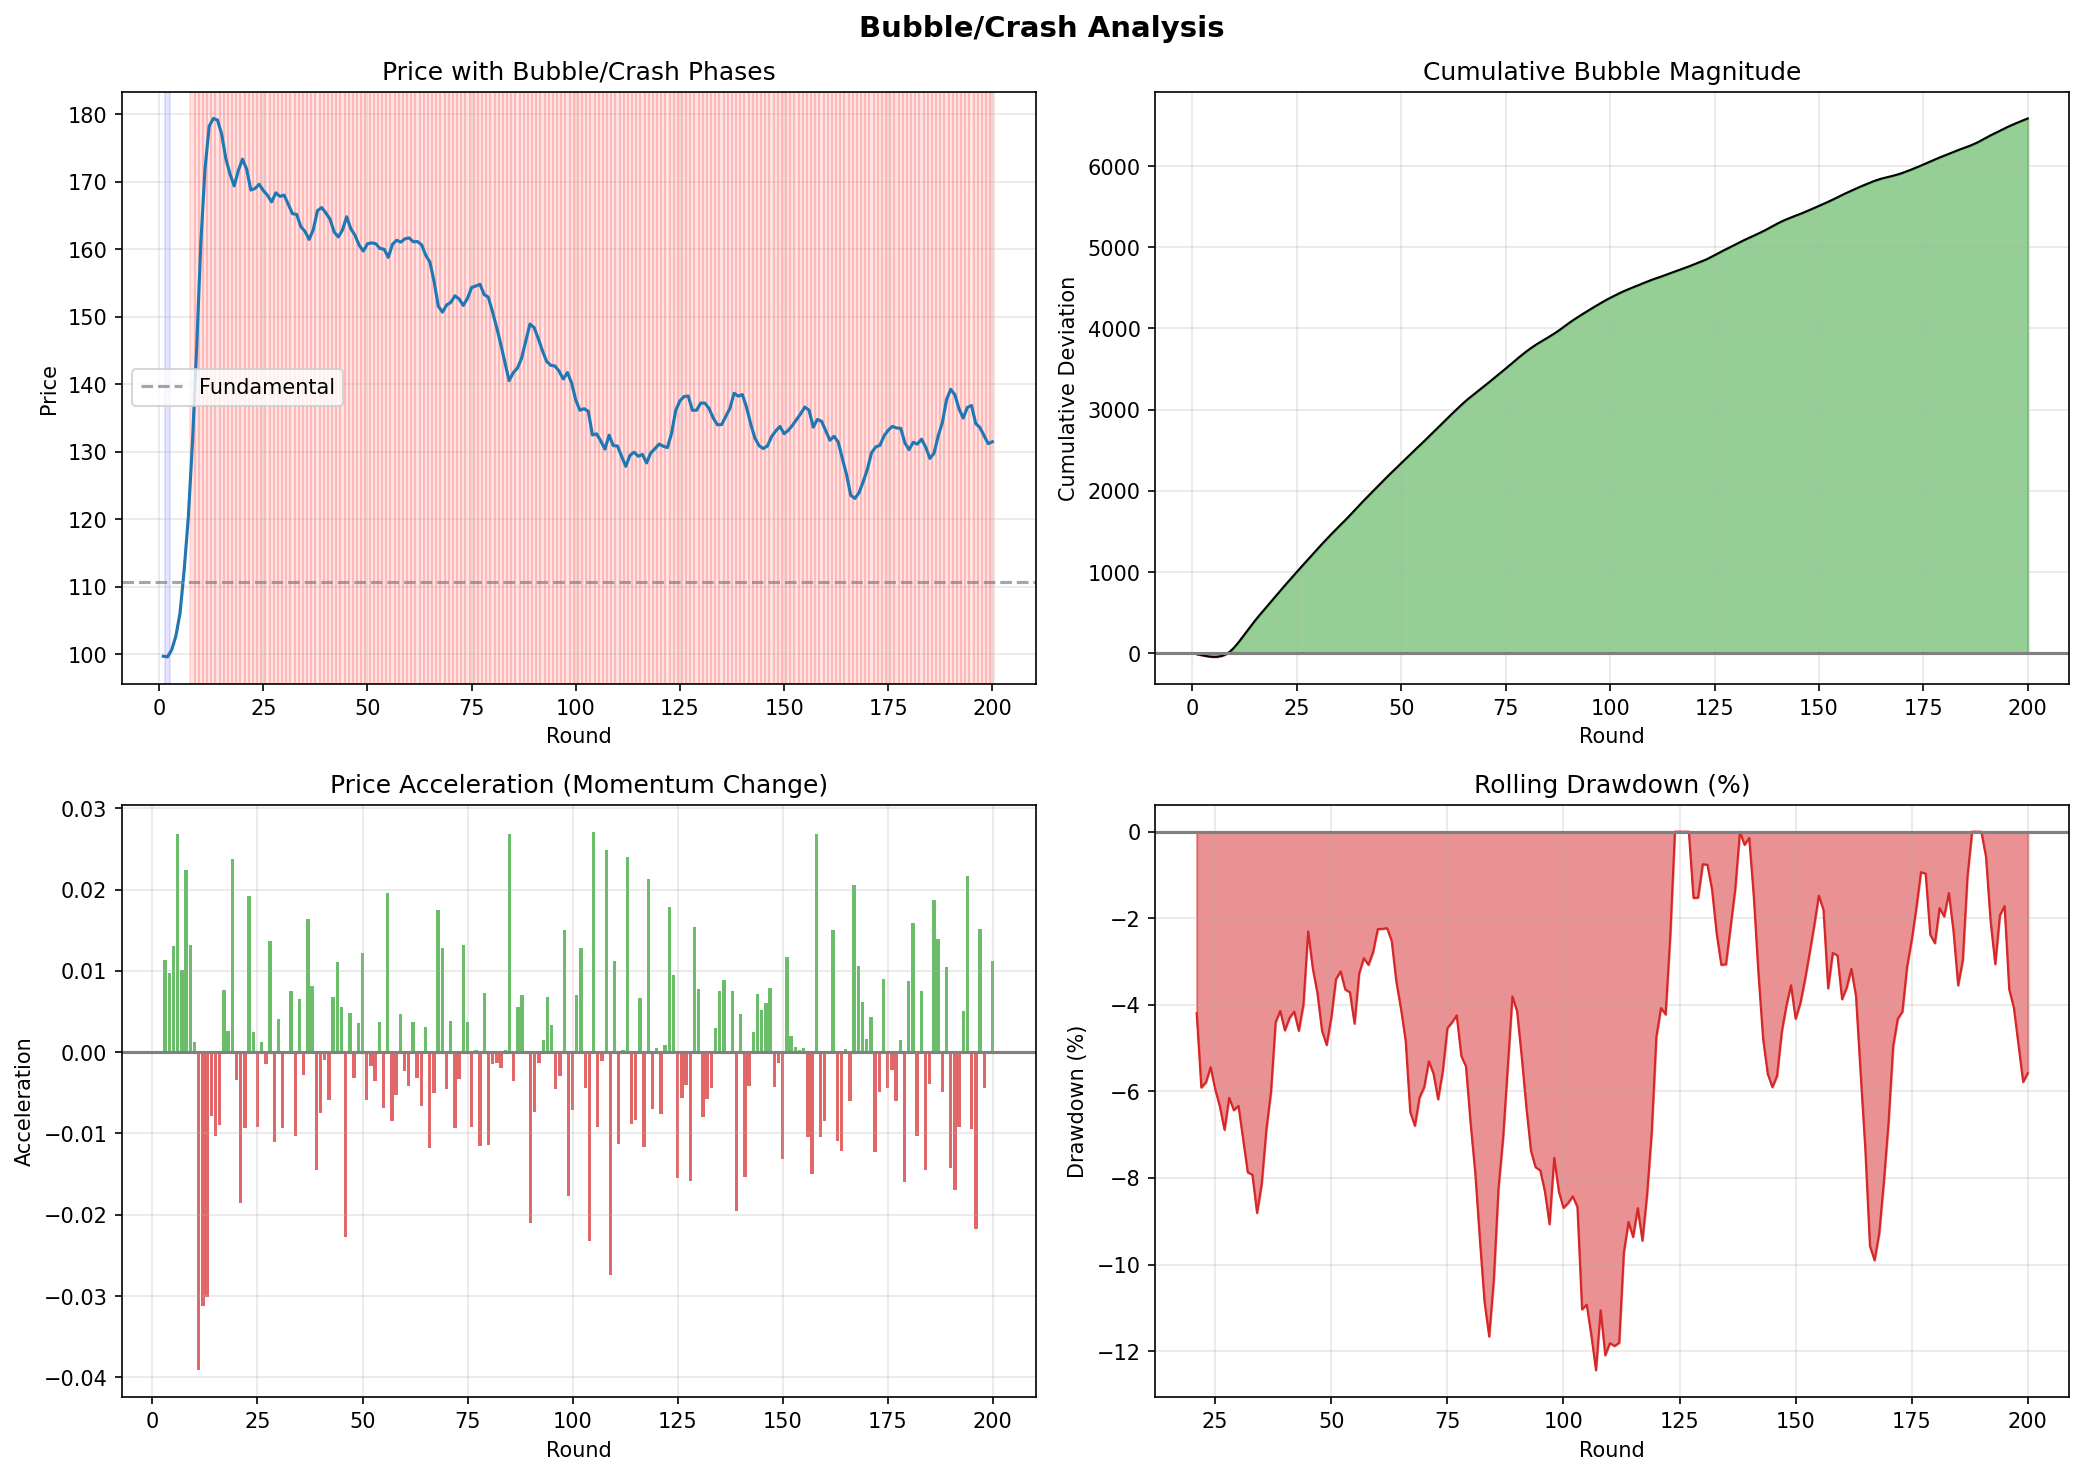
\includegraphics[width=\textwidth]{results/llm_results.jpg}
  \caption{Asset bubble simulation results using the LLM model.}
  \label{fig:llm}
\end{figure}

\paragraph{Results Analysis.}
The fundamental value is approximately 100. From the price trajectory, the market does not fluctuate stably around the fundamental value, but instead exhibits persistent deviation characteristics. The price repeatedly surges rapidly to levels significantly above fundamentals, accompanied by sharp pullbacks, forming a recurrent cycle of ``surge---retracement---resurge.'' This repetitive deviation pattern aligns with the basic features of asset bubble formation, namely ``price persistently deviating from fundamentals with deviation not dissipating in a single episode.''

From the decomposition results of deviation degree, overvaluation dominates, with deviation reaching substantial magnitudes across multiple phases---indicating that price premiums are not transient noise, but rather states accompanied by progressively accumulating bubble intensity. Meanwhile, deviation rapidly shifts to negative values after high-value phases, indicating that the system indeed possesses certain risk release and drawdown mechanisms.

Following bubble phases, the price does not exhibit rapid, sustained mean reversion after a single bubble burst. Although pronounced sharp drawdowns and deep plunges are observable, prices frequently revert to overvaluation intervals thereafter---resulting in insufficient post-burst recovery and recurrent reemergence of overvaluation states. Thus, compared to the classical path of ``bubble bursting leading to rapid bubble dissipation,'' this simulation more closely approximates a structure of alternating periodic bubbles and drawdowns: bubbles are not thoroughly liquidated, but instead undergo repeated high-level repricing and reaccumulation, causing cumulative bubble intensity to trend upward overall.

In summary, this simulation demonstrates sufficient bubble formation, with the market indeed exhibiting significant non-fundamental pricing and persistent overvaluation. However, bubble bursting remains incomplete, primarily manifested as recurrent overvaluation post-drawdown, rendering rapid bubble dissipation difficult. The likely causes are: excessive magnitude of random terms or exogenous shocks in the model, or imbalanced trader structure.


%%%%%%%%%%%%%%%%%%%%%%%%%%%%%%
%% Section 5: Future Plan
%%%%%%%%%%%%%%%%%%%%%%%%%%%%%%
\section{Future Plan}
\label{sec:future}

Building upon the preliminary understanding of large language models and their applications, we have identified certain limitations in parameter calibration that currently prevent precise replication of established financial theoretical models. The existing parameter configurations exhibit insufficient granularity in capturing the nuanced dynamics of bubble formation, propagation, and collapse mechanisms as prescribed by canonical asset pricing theory.

Moving forward, we intend to leverage the advanced capabilities of large language models---particularly their capacity for contextual reasoning, multi-agent simulation, and emergent behavior generation---to refine the parameterization framework. Specifically, we aim to:

\begin{itemize}[leftmargin=*]
  \item \textbf{Enhance Parameter Precision:} Utilize LLM-driven sensitivity analysis to identify critical thresholds for bubble ignition and bursting conditions, ensuring alignment with theoretical predictions regarding deviation persistence and mean reversion speeds.
  \item \textbf{Optimize Agent Heterogeneity:} Deploy LLMs to generate more sophisticated trader archetypes with heterogeneous belief formation processes, thereby improving the representation of sentiment-driven momentum and contrarian reversion dynamics.
  \item \textbf{Calibrate Shock Propagation:} Employ LLM-assisted scenario generation to model endogenous and exogenous shock distributions that more accurately trigger regime transitions between bubble accumulation and liquidation phases.
  \item \textbf{Validate Against Stylized Facts:} Implement iterative feedback loops wherein LLM-generated outputs are systematically benchmarked against empirical regularities of historical bubble episodes---such as super-exponential price growth, increasing volatility, and critical slowing down---to ensure behavioral and statistical fidelity.
\end{itemize}

Through these methodological advancements, we aspire to achieve simulation outputs that converge more tightly with theoretically expected ranges, thereby enhancing the explanatory and predictive power of the modeling framework for asset bubble phenomena.


%%%%%%%%%%%%%%%%%%%%%%%%%%%%%%
%% 5. Bibliography
%%%%%%%%%%%%%%%%%%%%%%%%%%%%%%
\bibliography{reference}
\bibliographystyle{iclr2026_conference}


\end{document}